% Titre de la premiere partie
\section{Introduction}
\subsection{Motivation}
%%%%%%%%%%%%%%%%%%%%%%%%%%%%%%%%%%%%%%%%%%%%%%%%
% Première diapo
%%%%%%%%%%%%%%%%%%%%%%%%%%%%%%%%%%%%%%%%%%%%%%%%
\begin{frame}{Limitations of Traditional Ways of Security}
\begin{itemize}
    \item<1-> Rapid 5G adoption increased connected devices, often with memory and energy constraints;
    \item<2-> Traditional security methods (e.g., public key cryptography) are impractical due to resource-intensive calculations;
    \item<3-> Inadequate security mechanisms in low-power/low-memory devices lead to fixed or low entropy keys, posing network vulnerabilities;
    \item<4-> PKC-based authentication fails to protect against person-in-the-middle attacks in short-range communications systems.
\end{itemize}


%\begin{itemize}
 %   \item<1-> The rapid adoption of 5G technology has led to a significant increase in the number of connected devices, many of which have constraints on memory and energy.
    
  %  \item<2-> Traditional security methods, such as public key cryptography (PKC), involve intensive calculations and require excessive resources for low-cost devices, making them impractical.
   % \item<3-> Inadequate security mechanisms for low-power/low-memory devices can result in fixed or low entropy keys, posing vulnerabilities to the entire network.
    %\item<4-> PKC-based authentication does not protect against person-in-the-middle attacks, which are prevalent in short-range communications systems like keyless entry and contactless payments.
 %\end{itemize}   
\end{frame}

\begin{frame}{PLS as a potential solution}
    Physical Layer Security (PLS) encompasses
    \begin{itemize}
        \item keyless PLS;
        \item key-based PLS;
        \item the recent branch of Physical Layer Authentication (PLA).
        \end{itemize}
    \begin{center}
        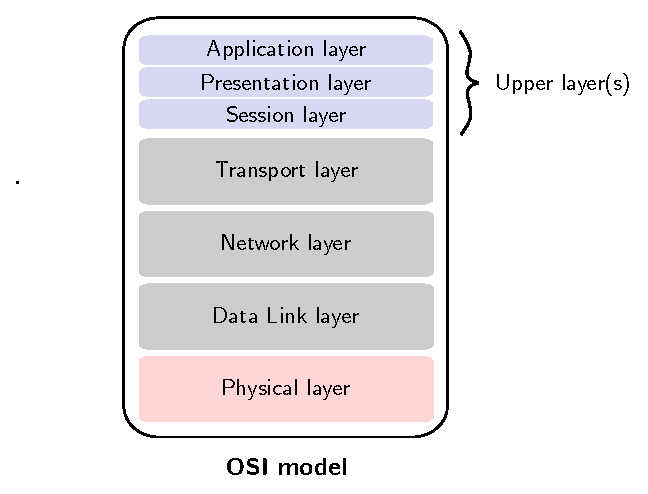
\includegraphics[width = 0.6\linewidth]{slides/figures/iso.eps}
        
    \end{center}
\end{frame}


%\begin{frame}
%\frametitle{PLS as a potential solution}

%\begin{itemize}
%\item<1-> Keyless PLS utilises the inherent randomness of the physical medium to achieve confidentiality without the need for keys or a secure key exchange.
%\item<2->Key-based PLS extracts unique randomness from the physical link to generate shared secret keys for symmetric cryptography.
%\item<3->PLA identifies devices based on hardware imperfections in transmitted signals and offers faster authentication before signal demodulation and decoding.

    
%\end{itemize}

%\end{frame}

%%%%%%%%%%%%%%%%%%%%%%%%%%%%%%%%%%%%%%%%%%%%%%%%
\subsection{Contributions}

\begin{frame}{Contributions}
\framesubtitle{...to the state-of-the-art of keyless PLS}
 \begin{itemize}
  \item<1-> Introducing a novel method, namely \textit{secret splitting}, that exploits base station cooperation for confidentiality;\\\hfill{(chapter~5)}
  \item<2-> Secrecy splitting addresses one of the most challenging requirements of keyless PLS: the need for a positive secrecy gap.\hfill{(chapter~5)}
 % \item<3-> Performing analytical analysis on the proposed scheme and deriving the optimal base station allocation.\hfill{(chapter~5)}
\item[\textcolor{blue}{$\rightarrow$}]<3-> \textcolor{blue}{1} peer-reviewed publication (GLOBECOM 2020)
 
\end{itemize}

\end{frame}

%%%%%%%%%%%%
\begin{frame}{Contributions}
\framesubtitle{...to the state-of-the-art of key-based PLS}

\begin{itemize}
    \item<1-> Revising secure distance for certain geometric environments; \hfill{(chapter~4)}
    \item<2-> Presenting a practical key agreement protocol for resource-constrained networks, successfully tested in an IoT network.\hfill{(chapter~7)}
    \item[$\rightarrow$]<3->\textcolor{blue}{2} peer-reviewed publications (VTC2022, ICC2023)
\end{itemize}

\end{frame}

\begin{frame}
\frametitle{Contributions}
\framesubtitle{...to the state of the art of physical layer authentication}
\begin{itemize}
    %\item<1-> Introducing a new concept for authenticating devices in short-range systems based on the spatial and temporal properties of the {RF} channel;\hfill{(chapter~6)}
    
    \item<1-> Proposing a scheme for secure authentication of co-located devices against distance fraud and replay attacks;
    \hfill{(chapter~6)}
    
    \item<2-> Proposing a scheme for validating the proximity of a non-powered device that communicates using backscattering modulation. \hfill{(chapter~6)}
    \item[\textcolor{blue}{$\rightarrow$}]<3-> \textcolor{blue}{2} peer-reviewed publications (VTC2021, WCNC2023) \& \textbf{1} patent (in collaboration with Toshiba).
\end{itemize}

\end{frame}

\iffalse
\begin{frame}{Publications}
    \begin{itemize}
    \item[1.] C. Paschou, O. Johnson, A. Doufexi, Z. Zhu, and W.H. Chin. ``Increasing the secrecy gap in quasi-static Rayleigh channels with secret splitting.'' In 2020 IEEE Globecom Workshops (GC Wkshps, pp. 1-7. IEEE, 2020. \hfill{[chapter~5]}

    \item[2.] C. Paschou, O. Johnson, Z. Zhu, and A. Doufexi. ``A Lightweight Protocol for Validating Proximity in UHF RFID Systems.'' In 2021 IEEE 94th Vehicular Technology Conference (VTC2021-Fall), pp. 1-7. IEEE, 2021. \hfill[chapter~6]
    
    \item[3.] C. Paschou, O. Johnson, Z. Zhu, and A. Doufexi.``Re-Defining Secure Distance for CSI-based Key Generation Protocols.'' In 2022 IEEE 95th Vehicular Technology Conference (VTC2022-Spring), pp. 1-6. IEEE, 2022.\hfill[chapter~4]
    \end{itemize}
    \end{frame}

\begin{frame}{Publications}
    \begin{itemize}
    \item[4.] C.Paschou, Z. Zhu, M. Sandell.
    ``Preventing replay/relay attacks in keyless entry systems.'' Patent 54322US, Oblon, McClelland, Maier \& Neustadt, {L.L.P.}, 2022. \hfill[chapter~6]
    
    
    \item[5.] C. Paschou, O. Johnson, Z. Zhu, and A. Doufexi. ``Physical Layer Protection Against Relay/Replay Attacks for Short-Range Systems.'' In 2023 IEEE Wireless Communications and Networking Conference (IEEE WCNC 2023), pp. 1-6. IEEE, 2023.\hfill[chapter~6]
    

    \item[6.] C. Paschou, F. Raimondo, M. Gugala, D. McEwan, J. Pope, G. Oikonomou.
    ``CRICKET: A Practical Physical Layer Key Agreement Protocol for IoT Networks.'' In 2023 IEEE International Conference of Communications (IEEE ICC 2023), pp. 1-7. IEEE, 2023.\hfill[chapter~7]
\end{itemize}
\end{frame}
 \fi
%\visible<3->{
%	\begin{figure}
%	\includegraphics[width=0.8\linewidth]{figures/Fig01}
%	\end{figure}
%	}

%%%%%%%%%%%%%%%%%%%%%%%%%%%%%%%%%%%%%%%%%%%%%%%%
% Troisième diapo
%%%%%%%%%%%%%%%%%%%%%%%%%%%%%%%%%%%%%%%%%%%%%%%%
\subsection*{}
\begin{frame}{Thesis Outline}
\begin{center}
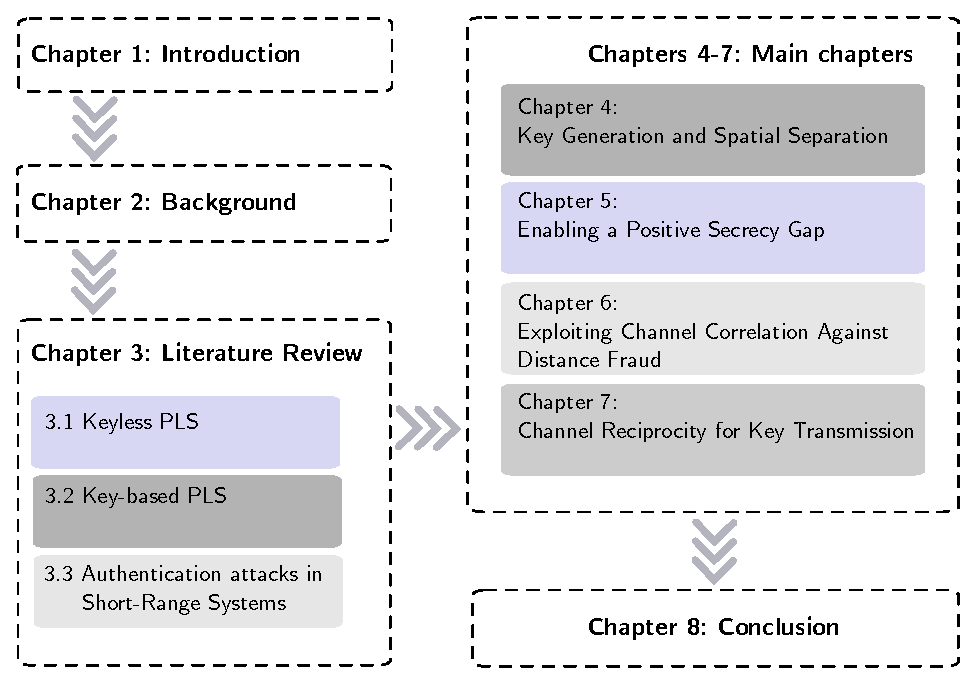
\includegraphics[width=0.9\linewidth]{slides/figures/outline.eps}
\end{center}

\end{frame}